\lab{Pandas III: Grouping and Presenting Data}{Pandas III: Grouping and Presenting Data}
\objective{Learn about Pivot tables, groupby, etc.}
\label{lab:pandas3}

MAJOR REVISIONS IN PROGRESS!!!!!!!!!!!!!!

\begin{comment}
This section will probably use 1-3 datasets from PyDataset describing diseases.
Since these datasets are easy to download and use, that will be a good way to compare how different datasets match certain plots better, and then similarly divide certain aspects of the data into different plots.

One example here will be the PyDataset's AIDS dataset.
In addition to its categories of infection and induction periods, we can compare adult cases to children using a bar chart, or simply focus on one of these two using a scatter plot.
There are many different ways to describe the data, here we will discuss how what we want to display effects the plot we choose.
\end{comment}

\section*{Introduction}
Pandas originated as a wrapper for numpy that was developed for purposes of data analysis. Data seldom comes in a format that is perfectly ready to use.  We always need to be able to interpret what our data is telling us.  Some data may be of little or no use, while other aspects of our data may be vital.  \emph{Pivoting} is an extremely useful way to sort through data and be able to present results clearly and compactly.  Two central ways to accomplish this are by using \li{groupby} and by using \emph{Pivot Tables}.

\section*{Groupby}

In Lab \ref{lab:pandas2} we introduced \li{pydatasets}, and mentioned how, in their raw format, plotting would be nonsensical.  Many datasets are simply composed of tables of individuals (represented as rows), with a list of classifiers associated with each one (columns).

For example, consider the \li{msleep} dataset.  In order to view the columns present in this dataset, we make use of the function \li{head()}.  This will show us the first five rows, and all of the columns.

\begin{lstlisting}
>>> import pandas as pd
>>> from pydataset import data
>>> msleep = data("msleep")
>>> msleep.head()
                         name       genus   vore         order  conservation  
1                     Cheetah    Acinonyx  carni     Carnivora            lc   
2                  Owl monkey       Aotus   omni      Primates           NaN   
3             Mountain beaver  Aplodontia  herbi      Rodentia            nt   
4  Greater short-tailed shrew     Blarina   omni  Soricomorpha            lc   
5                         Cow         Bos  herbi  Artiodactyla  domesticated   

   sleep_total  sleep_rem  sleep_cycle  awake  brainwt   bodywt  
1         12.1        NaN          NaN   11.9      NaN   50.000  
2         17.0        1.8          NaN    7.0  0.01550    0.480  
3         14.4        2.4          NaN    9.6      NaN    1.350  
4         14.9        2.3     0.133333    9.1  0.00029    0.019  
5          4.0        0.7     0.666667   20.0  0.42300  600.000 
\end{lstlisting}

Each row consists of a single type of mammal and its corresponding identifiers, including genus and order, as well as sleep measurements such as total amount of sleep (in hours) and REM sleep, in hours.
When we try to plot this data using plt.plot, the individual data points do not demonstrate overall trends.
\begin{lstlisting}
>>> msleep.plot(y="sleep_total", title="Mammalian Sleep Data", legend=False)
>>> plt.xlabel("Animal Index")
>>> plt.ylabel("Sleep in Hours")
>>> plt.show()
\end{lstlisting}
The above code results in Figure \ref{fig:sleep}.
\begin{figure}[H] 
    \centering
    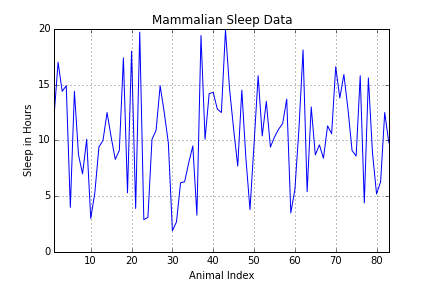
\includegraphics[width=.75\textwidth]{Msleep1.png}
    \caption{Source:  Proceedings of the National Academy of Sciences, 104 (3):1051-1056, 2007. Updates from V. M. Savage and G. B. West, with additional variables supplemented by Wikipedia.}
    \label{fig:sleep}
\end{figure}
This set of connected data points is not particularly revealing, as it plots the first numerical column, \li{sleep_total}, as a function of the animal index, which is seemingly random.

The \li{DataFrame} contains information that will help us to make better sense of this data.
Using \li{groupby()}, we can select the parts we want. As the name implies, \li{groupby()} takes a \li{DataFrame} and creates different groupings. For this dataset, let's consider the sleep differences between herbivores, omnivores, insectivores, and carnivores. To do so, we simply call the \li{groupby} method on the \li{vore} column to obtain a \li{groupby} object organized by diet classification.
\begin{lstlisting}
>>> vore = msleep.groupby("vore")
\end{lstlisting}
You can also group the data by multiple columns, for example, both the \li{vore} and \li{order} classifications.
To group and view this data, simply use:
\begin{lstlisting}
>>> vorder = msleep.groupby(["vore", "order"])

# View groups within vorder
>>> vorder.describe()
\end{lstlisting}
This listing is much too long to view here, but you should be able to see that it first sorts all rows into the appropriate \li{vore} category, and then into the appropriate \li{order} category.  It gives the count of rows in each section, along with the mean, standard deviation, and other potentially useful statistics.

Pandas \li{groupby} objects are not lists of new \li{DataFrames} associated with groupings.
They are better thought of as a dictionary or generator-like object which can be \emph{used} to produce the necessary groups.
However, the \li{get\_group()} method will do this, as follows:

\begin{lstlisting}
# Get carnivore group
>>> Carni = vore.get_group("carni")
# Get herbivore group
>>> Herbi = vore.get_group("herbi")
\end{lstlisting}

The \li{groupby} object includes many useful methods that can help us make visual comparisons between groups. 
The \li{mean()} method, for example, returns a new \li{DataFrame} consisting of the mean values attached to each group.
Using this method on our \li{vore} object returns a nicely organized \li{DataFrame} of the average sleep data for each mammalian diet pattern.
We can similarly create a \li{DataFrame} of the standard deviations for each group.

At this point, we have a nicely organized dataset that can easily be turned into a bar chart.
Here, we use the \li{DataFrame.loc} method to access three specific columns in the bar chart (\li{sleep_total}, \li{sleep_rem}, and \li{sleep_cycle}).
\begin{lstlisting}
>>> means = vore.mean()
>>> errors = vore.std()
>>> means.loc[:,["sleep_total", "sleep_rem", "sleep_cycle"]].plot(kind="bar", yerr=errors, title="Mean Mammallian Sleep Data")
>>> plt.xlabel("Mammal diet classification (vore)")
>>> plt.ylabel("Hours")
>>> plt.show()
\end{lstlisting}

\begin{figure}[H] 
    \centering
    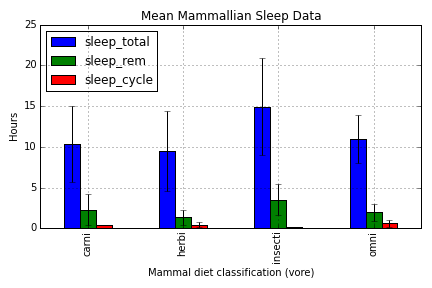
\includegraphics[width=.75\textwidth]{MeanMammal.png}
    \caption{Source:  Proceedings of the National Academy of Sciences, 104 (3):1051-1056, 2007. Updates from V. M. Savage and G. B. West, with additional variables supplemented by Wikipedia.}
    \label{fig:barplot}
\end{figure}

\begin{problem} 
Examine the \li{diamonds} dataset found in the \li{pydataset} module. 
This dataset contains the identifiers and attributes of 53,940  individual round cut diamonds. 
Using the \li{groupby} method, create three different visuals highlighting and comparing different aspects of the data.
This can be in the form of a single plot or comparative subplots.  Use the plotting techniques from Lab \ref{lab:pandas2}.

Print a few sentences for each plot explaining what type of graph you used, why, and what we learn about the dataset from your plot.
Don't forget to include titles, clear labels, and sourcing. 

The following is an example of comparative subplots, which may \emph{not} be used for your plots.
\begin{figure}[H] % Matplotlib vs. Pandas
    \centering
    \begin{minipage}[b]{0.48\textwidth}
    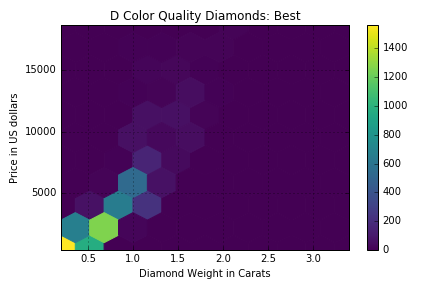
\includegraphics[width=\textwidth]{DiamondD.png}
    \end{minipage}
    \quad
    \begin{minipage}[b]{0.48\textwidth}
    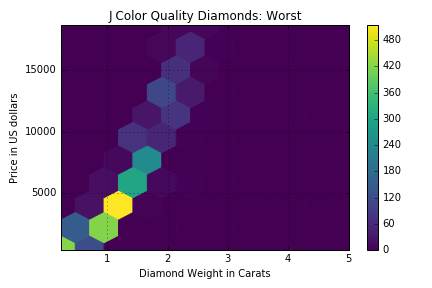
\includegraphics[width=\textwidth]{DiamondJ.png}
    \end{minipage}
    \caption{Source: Adopted from R Documentation}
    \label{fig:intro2}
\end{figure}

\begin{comment}
The code for the above figure is included here:
\begin{lstlisting}
>>> Diamonds = data("diamonds")
>>> DiaColor = Diamonds.groupby("color")
>>> Ddiamond = DiaColor.get_group("D")
>>> Jdiamond = DiaColor.get_group("J")

>>> Ddiamond.plot(kind="hexbin", x="carat", y="price", gridsize=10, title="D Color Quality Diamonds: Best", cmap="viridis")
>>> plt.ylabel("Price in US Dollars")
>>> plt.xlabel("Diamond Weight in Carats")
>>> plt.tight_layout()
>>> plt.show()

>>> Jdiamond.plot(kind="hexbin", x="carat", y="price", gridsize=10, title="J Color Quality Diamonds: Worst", cmap="viridis")
>>> plt.ylabel("Price in US Dollars")
>>> plt.xlabel("Diamond Weight in Carats")
>>> plt.tight_layout()
>>> plt.show()
\end{lstlisting}
\end{comment}

The following is an appropriate (if lengthy) description of our plots:
The above plots were created using \li{groupby} on the diamond colors and then using a hexbin comparing carats to price for the highest and lowest quality diamonds, respectively. 
This hexbin is particularly revealing for each set of thousands of diamonds because it meaningfully displays concentration of datapoints. 
Matplotlib's new \li{viridis} colorplot, with a dark background, reveals bins that would have been invisible with a white background.
By comparing these plots, we note that the greatest number of J quality diamonds in the dataset are about 1.25 carats and \$4000 dollars in price, whereas the highest concentration of D quality diamonds are smaller and therefore cheaper. 
We may attribute this to D quality diamonds being rarer, but the colorbar on the side reveals that D diamond numbers are, in fact, far higher than those of the J color. 
Instead it is simply more likely that D quality diamonds of larger sizes are rarer than those of smaller sizes. 
Both hexbins reveal a linearity between diamond weight and diamond price, with D diamonds showing more variability and J diamonds displaying a strict linearity.

\end{problem}

\li{Groupby} is a very useful method to order data.  However, it is not the perfect tool for every situation.  As we saw when sorting data by multiple columns, we can end up with a useful grouping, but too much information to display.  If we want to see information in table format, we can make use Pivot Tables.

\section*{Pivot Tables}
With a given pandas \li{DataFrame}, we can visualize data easily with the function \li{pivot_table()}. The Titanic dataset (\li{titanic.csv}) is especially apt for this.  It includes many columns, but we will use only those entitled``Survived", ``Pclass", ``Sex", ``Age", and ``Fare" here.  Once this has been loaded in, we can make Pivot Tables to view trends in the data.

\begin{lstlisting}
>>> titanic.pivot_table('Survived', index='Sex', columns='Pclass')
\end{lstlisting}

Here ``value'' is the category (or column in the original datset) we want to compare, ``index'' will be the category for the row of our pivot table, and ``columns'' is the category to organize as the columns for our pivot table.

Let's say we want to further break down the survival rates to compare how different ages fared in the voyage, according to their gender and class. We could be asking ourselves the question, ``What about the children? Were male children really that likely to die as compared to female children?''. As you will see with pivot tables, as we see these simple breakdowns of the data, more questions can, and should arise. You should consistently ask yourself questions about the relevance of the numbers you see in the pivot tables you create. So let's look at how age was a factor in survival.

Noting that in the original dataset, the `age' column has an integer value for the age of each passenger, if we were to just add `age' as an argument for index, then the table would create a new row for EACH age present. This wouldn't be a very useful or simple table to visualize, so we desire to partition the ages into 3 categories. We use the function \li{cut()} to do this.

\begin{lstlisting}
>>> # Partition each of the passengers into 3 categories based on their age
>>> age = pd.cut(titanic['age'], [0,12,18,80])
\end{lstlisting}

Now with this other partition of the column age, we can add this dimension to our pivot table, passing it along with `sex' in a list to the parameter index.

\begin{lstlisting}
>>> # Add a third dimension, age, to our pivot table
>>> titanic.pivot_table('survived', index =['sex', age], columns='class')
\end{lstlisting}

Add table
%\begin{figure}
%    \centering
%    \includegraphics[width=.75\textwidth]{piv_gend_class_age.pdf}
%\end{figure}

What do we notice? First of all, male children (ages 0 to 12) in 1st and 2nd class were very likely to survive, whereas those in 3rd class did not. However, look at the female children in first class. 0 percent of them survived? This might seem a little odd, but if we looked at our data set again to see how many passengers fell into this category of female, 1st class, and age 0 to 12, we would find only 1 passenger. Therefore, the statistic that 0\% of female children in first class died is misleading. We can visualize this by specifying the parameter aggfunc=`count'.

\begin{lstlisting}
>>> titanic.pivot_table('survived', columns='sex', index=['class',age], aggfunc='count')
\end{lstlisting}

Add table
%\begin{figure}
%    \centering
%    \includegraphics[width=.75\textwidth]{piv_gca_count.pdf}
%\end{figure}

The parameter aggfunc defaults to `mean', which is why we have seen the mean survival rate for each of the different categories. By specifying aggfunc to be `count', we get how many passengers of each category are present in the table. In this case, specifying the value is `survived' is redundant.

This brings up another point about these datasets. We note for this dataset, we have roughly 800 passengers' data. This is not that large of a data set relatively, and we aren't guaranteed significant sample sizes for each possible partitioning of the the data columns. This is important to keep in mind with any dataset, and you should always ask questions about the numbers you see in pivot tables before making any conclusions.

Now, for fun, let's add a fourth dimension to our table- the cost of the passenger's ticket. Let's add this dimension to our columns of the pivot table. We now use the function \li{qcut()} to partition the fare column's data into two different categories.

With this partition we add this dimension to columns, passing fare and `class' in as a list to the argument ``columns".

\begin{lstlisting}
>>> # Partition fare column into 2 categories based on the values present in fare column
>>> fare = pd.qcut(titanic['fare'], 2)
>>> # Add the fare as a dimension of columns
>>> titanic.pivot_table('survived', index=['sex',age], columns=[fare, 'class'])
\end{lstlisting}

Add table
%\begin{figure}
%    \centering
%    \includegraphics[width=.75\textwidth]{fare_splice.pdf}
%\end{figure}

We now see something else about our dataset - we get NaNs in some entries. The dataset has some invalid entries or incomplete data for the column fare. Let's investigate further.

By inspecting our dataset, we can see that there might not be any people in the categories given in the pivot table. We can fill in the NaN values in the pivot table with the argument \li{fill_value}. We show this below.

\begin{lstlisting}
>>> # Specify fill_value = 0.0
>>> titanic.pivot_table('survived', index=['sex',age], columns=[fare, 'class'], fill_value=0.0)
\end{lstlisting}

Add table
%\begin{figure}
%    \centering
%    \includegraphics[width=.75\textwidth]{fill_zeros.pdf}
%\end{figure}

It should be noted though that with datasets where NaN's occur frequently, some preprocessing needs to be done so as to get the most accurate statistics and insights about your dataset. You should've worked on cleaning datasets in previous lab, so we don't go further into detail about the topic here.

\begin{problem}
Suppose that someone claims that the city from which a passenger embarked had a strong influence on the passenger's survival rate. Investigate this claim.
\begin{enumerate}
\item Using a \li{groupby()} call, see what the survival rates of the passengers were based on where they embarked from (\li{embark_town}).
\item Next, create a pivot table to further look at survival rates based on both place of embarkment and gender.
\item What do these tables suggest to you about the significance of where people embarked in influencing their survival rate? But in light of the context of the problem, what do you think this really means? Find 2 more pivot tables that investigate the claim further, looking at other criterion (e.g., class, age, etc.).
\end{enumerate}
\end{problem}












